\section{Complex Numbers}

\begin{frame}{Representing Complex Numbers}
    \begin{columns}[T]
        \begin{column}{0.5\textwidth}
            The \alert{Cartesian} or \alert{rectangular} form:
            \begin{equation*}
                z = x + jy,
            \end{equation*}
            where $j = \sqrt{-1}$ and $x$ and $y$ are real numbers referred to respectively as the real part and the imaginary part. I.e.,
            \begin{equation*}
                x = \mathfrak{Re}\{z\}, y = \mathfrak{Im}\{z\}
            \end{equation*}
            The \alert{polar} form:
            \begin{equation*}
                z = re^{j\theta},
            \end{equation*}
            where $r>0$ is the \alert{magnitude} of $z$ and $\theta$ is the \alert{angle} or \alert{phase} of $z$.
            \begin{equation*}
                r = |z|, \theta = \sphericalangle z.
            \end{equation*}
        \end{column}
        \pause
        \begin{column}{0.5\textwidth}
            The relationship between these two representations can be determined from \alert{Euler's relation}:
            \begin{equation*}
                e^{j\theta} = \cos\theta + j\sin\theta
            \end{equation*}
            or by plotting $z$ in the complex plane.
                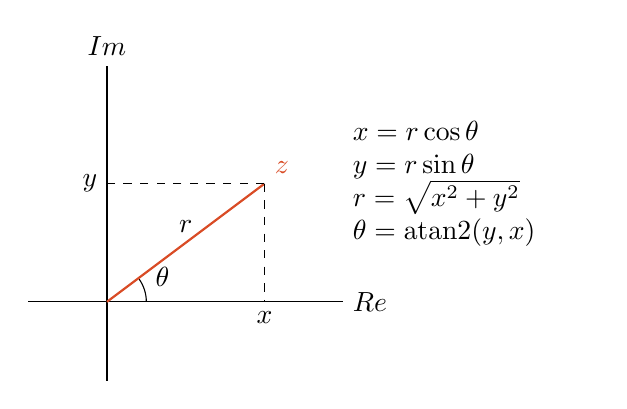
\begin{tikzpicture}
                	\draw (-1,0) -- (3,0) node [anchor=west] {$\mathfrak{Re}$};
                	\draw (0,-1) -- (0,3) node [anchor=south] {$\mathfrak{Im}$};
                	\draw[thick, red!40!brown] (0,0) -- (2, 1.5) node[midway, above, black] {$r$}  coordinate (z) node [anchor=south west] {$z$};
                	\draw[dashed] (z) -- ++(0, -1.5) node[anchor=north] {$x$};
                	\draw[dashed] (z) -- ++(-2,0) node[anchor=east] {$y$};	
                	\draw (0.5, 0) arc (0:35:0.5) node [near start, anchor=south west] {$\theta$};
                    \node at (3,1.5) [anchor=west, text width=3cm] {$x = r\cos\theta$\\$y=r\sin\theta$\\$r = \sqrt{x^2+y^2}$\\$\theta = \mathrm{atan2}(y,x)$};
                \end{tikzpicture}
        \end{column}
    \end{columns}
\end{frame}


\begin{frame}
    \begin{columns}[T]
        \begin{column}{0.5\textwidth}
            {\bf Example} Let $z_0$ be a complex number with polar coordinates $(r_0, \theta_0)$ and Cartesian coordinates $(x_0, y_0)$. Determine expressions for the Cartesian coordinates of the following complex numbers in terms of $x_0$ and $y_0$. Plot the points $z_0, z_1, z_2, z_3, z_4$, and $z_5$ in the complex plane when $r_0 = 2$ and $\theta_0 = \pi/4$ and when $r_0 = 2$ and $\theta_0 = \pi/2$. Indicate on the plot the real and imaginary parts of each point.
            \begin{enumerate}[<alert@+>]
                \item $z_1 = r_0e^{-j\theta_0}$
                \item $z_2 = r_0$
                \item $z_3 = r_0e^{j(\theta_0 + \pi)}$
                \item $z_4 = r_0e^{j(-\theta_0 + \pi)}$
                \item $z_5 = r_0e^{j(\theta_0 + 2\pi)}$
            \end{enumerate}

        \end{column}
            \begin{column}{0.5\textwidth}
            \begin{align*}
                z_0 &= r_0e^{j\theta_0} = r_0(\cos\theta_0 + j\sin\theta_0)\\ &= r_0\cos\theta_0 + jr_0\sin\theta_0 = x_0 + jy_0.
            \end{align*}
            \onslide<1->
            \begin{equation*}
                z_1 = r_0e^{-j\theta} = r_0(\cos(-\theta_0) + j\sin(-\theta_0)) = x_0 - jy_0.
            \end{equation*}
            \onslide<2->
            \begin{equation*}
                z_2 = r_0 = \sqrt{x_0^2+y_0^2}
            \end{equation*}
            \onslide<3->
            \begin{align*}
                z_3 &= r_0e^{j(\theta_0 + \pi)}\\&= r_0(\cos(\theta_0 + \pi) + \sin(\theta_0 + \pi)) = -x_0 - jy_0 = -z_0.
            \end{align*}
            \onslide<4->
            \begin{equation*}
                z_4 = -x_0 + jy_0.
            \end{equation*}
            \onslide<5->
            \begin{equation*}
                z_5 = z_0.
            \end{equation*}
        \end{column}
    \end{columns}
\end{frame}


\begin{frame}{$r=2, \theta = \pi/4$}
    $z_1 = r_0e^{-j\theta_0}$, $z_2 = r_0$, $z_3 = r_0e^{j(\theta_0 + \pi)}$, $z_4 = r_0e^{j(-\theta_0 + \pi)}$, $z_5 = r_0e^{j(\theta_0 + 2\pi)}$
    \begin{tikzpicture}
        	\draw (-3,0) -- (3,0) node [anchor=west] {$\mathfrak{Re}$};
        	\draw (0,-3) -- (0,3) node [anchor=south] {$\mathfrak{Im}$};
    	\node [red!20!brown] at (45:2) {$\times$};    	
        	\node at (45:2) [anchor=west] {\scriptsize $z_0, z_5 \equiv (\sqrt{2}, \sqrt{2})$};
        	\node [red!20!brown] at (225:2) {$\times$};
        	\node at (225:2) [anchor=east] {\scriptsize $z_3 \equiv (-\sqrt{2}, -\sqrt{2})$};
        	\node [red!20!brown] at (135:2) {$\times$};
        	\node at (135:2) [anchor=east] {\scriptsize $z_4 \equiv (-\sqrt{2}, \sqrt{2})$};    	
        	\node [red!20!brown] at (-45:2) {$\times$};
        	\node at (-45:2) [anchor=west] {\scriptsize $z_1 \equiv (\sqrt{2}, -\sqrt{2})$};    	    	
        	\begin{scope}[xshift=7cm]
    	    	\draw (-3,0) -- (3,0) node [anchor=west] {$\mathfrak{Re}$};
    	    	\draw (0,-3) -- (0,3) node [anchor=south] {$\mathfrak{Im}$};
    	    	\draw (0,0) circle (2);
    	    	\node at (30:2) [anchor=west] {$z_2$};    		
        	\end{scope}
    \end{tikzpicture}
\end{frame}

\begin{frame}{$r=2, \theta = \pi/2$}
    $z_1 = r_0e^{-j\theta_0}$, $z_2 = r_0$, $z_3 = r_0e^{j(\theta_0 + \pi)}$, $z_4 = r_0e^{j(-\theta_0 + \pi)}$, $z_5 = r_0e^{j(\theta_0 + 2\pi)}$
    \begin{tikzpicture}
        	\draw (-3,0) -- (3,0) node [anchor=west] {$\mathfrak{Re}$};
        	\draw (0,-3) -- (0,3) node [anchor=south] {$\mathfrak{Im}$};
    	\node [red!20!brown] at (-90:2) {$\times$};    	
        	\node at (-90:2) [anchor=west] {\scriptsize $z_1, z_3 \equiv (0, -2)$};
       	
        	\node [red!20!brown] at (90:2) {$\times$};
        	\node at (90:2) [anchor=west] {\scriptsize $z_0, z_4, z_5 \equiv (0, 2)$};    	    	
        	\begin{scope}[xshift=7cm]
    	    	\draw (-3,0) -- (3,0) node [anchor=west] {$\mathfrak{Re}$};
    	    	\draw (0,-3) -- (0,3) node [anchor=south] {$\mathfrak{Im}$};
    	    	\draw (0,0) circle (2);
    	    	\node at (30:2) [anchor=west] {$z_2$};    		
        	\end{scope}
    \end{tikzpicture}
\end{frame}


\begin{frame}
    \begin{columns}[T]
        \begin{column}{0.3\textwidth}
            Express each of the following complex numbers in polar form, and plot them in the complex plane, indicating the magnitude and angle of each number.
            \begin{enumerate}[<alert@+>]
                \item $1 + j\sqrt{3}$
                \item $-5$
                \item $-5 -5j$
                \item $3+4j$
                \item $(1-j\sqrt{3})^3$
                \item $\dfrac{e^{j\pi/3}-1}{1+j\sqrt{3}}$
            \end{enumerate}

        \end{column}
        \begin{column}{0.7\textwidth}
        \begin{overprint}
        \onslide<1>
                \begin{align*}
                  1 + j\sqrt{3} &= \sqrt{1^2 + (\sqrt{3})^2}\left(\dfrac{1}{\sqrt{1^2 + (\sqrt{3})^2}} + j\dfrac{\sqrt{3}}{\sqrt{1^2 + (\sqrt{3})^2}}\right) \\
                   &= 2e^{j\mathrm{atan2}(\sqrt{3}, 1)} \\
                   &= 2e^{j\pi/3}
                \end{align*}

                \begin{tikzpicture}
                	\draw (-2,0) -- (2,0) node [anchor=west] {$\mathfrak{Re}$};
                	\draw (0,-2) -- (0,2) node [anchor=south] {$\mathfrak{Im}$};
                    \draw[red!50!black, thick] (0,0) -- (60:1.5) node[midway, above] {$2$} node[anchor=west] {$1 + j\sqrt{3}$};
                    \draw[draw=green!20!black, -latex] (0.5, 0) arc (0:60:0.5) node [near start, anchor=south west] {$\pi/3$};
                \end{tikzpicture}
        \onslide<2>
                \begin{align*}
                  -5 &= 5(-1 + j0) \\
                   &= 5e^{j\mathrm{atan2}(0, -1)} \\
                   &= 5e^{j\pi}
                \end{align*}

                \begin{tikzpicture}
                	\draw (-2,0) -- (2,0) node [anchor=west] {$\mathfrak{Re}$};
                	\draw (0,-2) -- (0,2) node [anchor=south] {$\mathfrak{Im}$};
                    \draw[red!50!black, thick] (0,0) -- (180:1.5) node[midway, above] {$5$} node[anchor=south east] {$-5$};
                    \draw[draw=green!20!black, -latex] (0.5, 0) arc (0:180:0.5) node [near start, anchor=south west] {$\pi$};
                \end{tikzpicture}

        \onslide<3>
                \begin{align*}
                  -5 -5j &= 5(-1 + j(-1)) \\
                   &= 5e^{j\mathrm{atan2}(-1, -1)} \\
                   &= 5e^{-j3\pi/4}
                \end{align*}

                \begin{tikzpicture}
                	\draw (-2,0) -- (2,0) node [anchor=west] {$\mathfrak{Re}$};
                	\draw (0,-2) -- (0,2) node [anchor=south] {$\mathfrak{Im}$};
                    \draw[red!50!black, thick] (0,0) -- (-135:1.5) node[midway, above, xshift=-0.2cm] {$5\sqrt{2}$} node[anchor=north] {$-5-j5$};
                    \draw[draw=green!20!black, -latex] (0.5, 0) arc (0:-135:0.5) node [midway, anchor=north west] {$-3\pi/4$};
                \end{tikzpicture}
        \onslide<4>
                \begin{align*}
                  3 +4j &= 5(3/5 + j4/5) \\
                   &= 5e^{j\mathrm{atan2}(4, 3)} \\
                   &= 5e^{-j3\pi/4}
                \end{align*}

                \begin{tikzpicture}
                	\draw (-2,0) -- (2,0) node [anchor=west] {$\mathfrak{Re}$};
                	\draw (0,-2) -- (0,2) node [anchor=south] {$\mathfrak{Im}$};
                    \draw[red!50!black, thick] (0,0) -- (53.1:1.5) node[midway, above, xshift=-0.2cm] {$5$} node[anchor=south] {$3+4j$};
                    \draw[draw=green!20!black, -latex] (0.5, 0) arc (0:53.1:0.5) node [midway, anchor= west] {$53.1^\circ$};
                \end{tikzpicture}
        \onslide<5>
                \begin{align*}
                  (1-j\sqrt{3})^3 &= \left(2e^{-j\pi/3}\right)^3 \\
                   &= 8e^{-j\pi} \\
                \end{align*}

                \begin{tikzpicture}
                	\draw (-2,0) -- (2,0) node [anchor=west] {$\mathfrak{Re}$};
                	\draw (0,-2) -- (0,2) node [anchor=south] {$\mathfrak{Im}$};
                    \draw[red!50!black, thick] (0,0) -- (-180:1.5) node[midway, above, xshift=-0.2cm] {$8$} node[anchor=south east] {$(1-j\sqrt{3})^3$};
                    \draw[draw=green!20!black, -latex] (0.5, 0) arc (0:-180:0.5) node [midway, anchor= north] {$-\pi$};
                \end{tikzpicture}
        \end{overprint}
        \end{column}
    \end{columns}
\end{frame}

\begin{frame}{$\cos\theta$ and $\sin\theta$}
    Using Euler's relations, derive the following relationships:
    \begin{enumerate}
        \item $\cos\theta = \frac{1}{2}(e^{j\theta} + e^{-j\theta})$
        \item $\sin\theta = \frac{1}{2j}(e^{j\theta} - e^{-j\theta})$
    \end{enumerate}
    \begin{columns}[t]
        \begin{column}{0.5\textwidth}
            \pause
            \begin{align*}
                e^{j\theta}&= \cos\theta +  j\sin\theta\\
                e^{-j\theta}&= \cos\theta -  j\sin\theta\\
            \end{align*}
            \pause
            Adding
            \begin{align*}
                e^{j\theta} + e^{-j\theta}&= 2\cos\theta \\
                \cos\theta &= \frac{1}{2}(e^{j\theta} + e^{-j\theta})\\
            \end{align*}
        \end{column}
        \begin{column}{0.5\textwidth}
            \pause
            Subtracting
            \begin{align*}
                e^{j\theta} - e^{-j\theta}&= 2j\sin\theta \\
                \sin\theta &= \frac{1}{2j}(e^{j\theta} - e^{-j\theta})\\
            \end{align*}
        \end{column}
    \end{columns}


\end{frame}


\begin{frame}{Complex Conjugate}
    Let $z$ denote a complex variable; i.e.,
    \begin{equation*}
        z = x + jy = re^{j\theta}.
    \end{equation*}
    The \alert{complex conjugate} of $z$ is
    \begin{equation*}
        z^\ast = x - jy = re^{-j\theta}.
    \end{equation*}
\end{frame}

\begin{frame}
    Show that
    \begin{enumerate}
      \item $zz^\ast = r^2$
      \item $z + z^\ast = 2\mathfrak{Re}\{z\}$
      \item $z - z^\ast = 2j\mathfrak{Im}\{z\}$
    \end{enumerate}
    \pause
    \begin{enumerate}
      \item $zz^\ast = re^{j\theta}re^{-j\theta} = r^2e^0 = r^2$
      \item $ z + z^\ast  = x + jy + x - jy  = 2x = 2\mathfrak{Re}\{z\}$
      \item $ z - z^\ast  = x + jy - (x - jy)  = 2jy = 2j\mathfrak{Im}\{z\}$
    \end{enumerate}
    \pause
    List the values of
    \begin{overprint}
        \onslide<3>
        \begin{enumerate}
          \item $e^{j0}$
          \item $e^{j\pi/2}$
          \item $e^{j\pi}$
          \item $e^{j3\pi/2}$
          \item $e^{j2\pi}$
        \end{enumerate}
        \onslide<4>
        \begin{enumerate}
          \item $e^{j0} = 1$
          \item $e^{j\pi/2} = j$
          \item $e^{j\pi} = -1$
          \item $e^{j3\pi/2} = -j$
          \item $e^{j2\pi} = 1$
        \end{enumerate}
    \end{overprint}

\end{frame} 